\documentclass{article}

\usepackage{lipsum}
\usepackage[margin=2cm, left=2cm, includefoot]{geometry}
\usepackage{graphicx}
\usepackage{float}
\usepackage{hyperref}
\usepackage{pdflscape}

% Header and footer
\usepackage{fancyhdr}
\pagestyle{fancy}
\setcounter{secnumdepth}{4}

\rhead{}
\lhead{}
\fancyfoot{}
\fancyfoot[R]{\thepage}
\renewcommand{\headrulewidth}{0pt}
\renewcommand{\footrulewidth}{0pt}
\let\cleardoublepage\clearpage
%

\begin{document}
	
	\begin{titlepage}
		\begin{center}
			\line(1,0){500}\\
			[6mm]
			\huge{\bfseries Software Requirements Specification}\\
			\line(1,0){500}\\
			[5mm]
			
\includegraphics[width=150px]{../images/AWorldOfPlants.png}
			\\
			[5mm]
			\large\textbf{Project:}\\A World of Things\\
			[3mm]
			\large\textbf{Client:}\\Julian Hambleton-Jones\\
			[3mm]
			\large \textbf{Team:}\\Funge\\
			\line(1,0){500}\\
			[5mm]
			\large \textbf{Team Members:}\\
			[3mm]
			\large 14214742 - Matthew Botha\\
			\large 14446619 - Gian Paolo Buffo\\
			\large 14027021 - Matthias Harvey\\
			\large 14035538 - Dillon Heins\\[3mm]
		\end{center}
	\end{titlepage}
	
	\cleardoublepage
	\thispagestyle{empty}
	\tableofcontents
	\begin{table}[]
\centering
\caption{Version Table}
\label{my-label}
\begin{tabular}{|l|l|l|ll}
\cline{1-3}
\textbf{Version} & \textbf{Date} & \textbf{Description}                                                                                                                                                                                                               &  &  \\ \cline{1-3}
0.1              & 22/05/2016    & \begin{tabular}[c]{@{}l@{}}Vision, scope, architectural requirements\\ and initial architecture design.\end{tabular}                                                                                                               &  &  \\ \cline{1-3}
0.2              & 29/07/2016    & \begin{tabular}[c]{@{}l@{}}Creation of separate documents for architecture\\ design, software requirements, testing and user \\ manual. Each populated with the relevant\\ information for the project at this stage.\end{tabular} &  &  \\ \cline{1-3}
0.3              & 11/09/2016    & \begin{tabular}[c]{@{}l@{}}Remake of all documents. Combination of them\\ into a single document. Documents follow\\ guidelines as discussed with lecturer.\end{tabular}                                                           &  &  \\ \cline{1-3}
\end{tabular}
\end{table}
	
	\cleardoublepage
	\setcounter{page}{1}
	
	\textit{Disclaimer: The system is still under development. All documentation will be updated as the system progresses}

\section{Introduction}
	\subsection{General Uses}
		\begin{itemize}
			\item Registering of a user
			\item Providing user with temporary credentials when they login
			\item Managing of unauthenticated and authenticated processes
			\item Ability to create a plant object and associate it with the logged in user
			\item Association of plant objects with IoT devices
			\item Analysis of data received from devices through means of graphs
			\item Management of hardware such as pumps and RGB LEDs
			\item Ability to update plant objects
			\item Ability to delete plant object
		\end{itemize}
	\subsection{Purpose}
		This document serves to explore the details and requirements of the 'A World of Plants' system. This is including
but not limited to the overall features of the system, interfaces, functionality, constraints and integration. This document is to serve as a reference tool for developers and as an informative resource for clients. Any third party collaborators who may have a need to use a reference to the 'A World of Plants' system may also refer to this document for reference.
	\subsection{Structure}
		This document covers the software requirement specifications for the 'A World of Plants' project. It covers the vision, background, scope, functional requirements and application design, use cases and services contracts, required functionality, process specifications, domain models, and open issues.

\section{Vision}
The aim of this project is to build an innovative Internet of Things solution through the use of the Amazon Web Services Internet of Things hardware platform as well as the Amazon Web Services Cloud. No problem was formally defined and hence it was up to us to determine what solution we would be creating. We opted to create a solution which focuses on the education of students with regard to agriculture and plant sciences.\\\\
We plan to motivate students to become interested in agriculture by creating an "Internet of Plants". This involves the networking and monitoring of living plants in order to analyse aspects of their environment - such as water intake, lighting, humidity, moisture, mineral composition and temperature. These results will be used to create a collaborative platform on which users may share their own results and learn from the results of others, in order to grow the best possible plants. The main purpose of the platform is to encourage younger generations to become interested in agriculture and, in doing so, help stimulate South Africa's agricultural industry.\\\\
We plan to implement gamification on our platform as a way to encourage competition amongst users. Given enough time, we would like to automate more parts of the system - such as automated watering. Additionally, AI learning could be employed to optimise the conditions under which plants grow. By combining automation and AI learning, we could create an interesting challenge for the users: Grow a plant better than our control plant grown with the help of AI.

\section{Background}
This project is part of a Software Engineering module (COS 301) for the University of Pretoria. Our client is Julian Hambleton-Jones and our project was to create anything we wanted using the AWS IoT platform. What we decided upon was the creation of a network of living plants which are to be analysed and looked after through the use of IoT devices and our software system.
	
\cleardoublepage
\section{Scope}
	\subsection{Plants Monitoring and Environment Control}
		The scope of the \emph{Plants Monitoring and Environment Control} module is shown below in Figure 1.
		
		\begin{figure}[H]
			\centering
			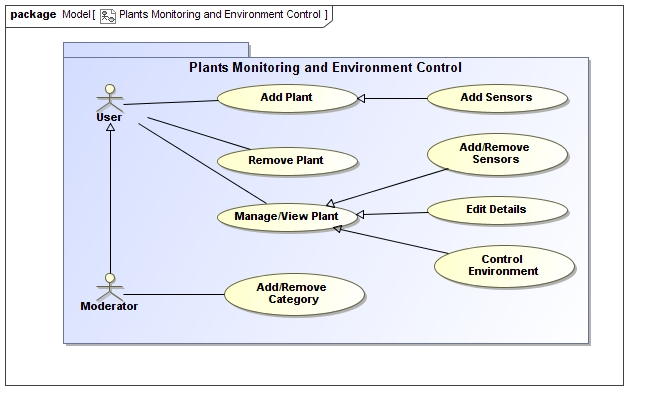
\includegraphics[width=\textwidth]{../software-architecture-specification/Plants_Monitoring_and_Environment_Control.jpg}
			\caption{The scope of functionality required from the \emph{Plants Monitoring and Environment Control} module}
		\end{figure}
		
		The scope of the \emph{Plants Monitoring and Environment Control} module includes:
		
		\begin{itemize}
			\item Adding a plant, which includes adding sensors to the plant object.
			\item Removing plants from the system, which will remove the plant object from the current plant view, but not from the database.
			\item Managing and viewing current plants' details and settings, which includes adding and removing sensors, editing plant details and changing the environment control parameters.
			\item Adding and removing categories of plants, which can only be done by a moderator.
		\end{itemize}
		
	\pagebreak
	\subsection{People}
		The scope of the \emph{People} module is shown below in Figure 2.
		
		\begin{figure}[H]
			\centering
			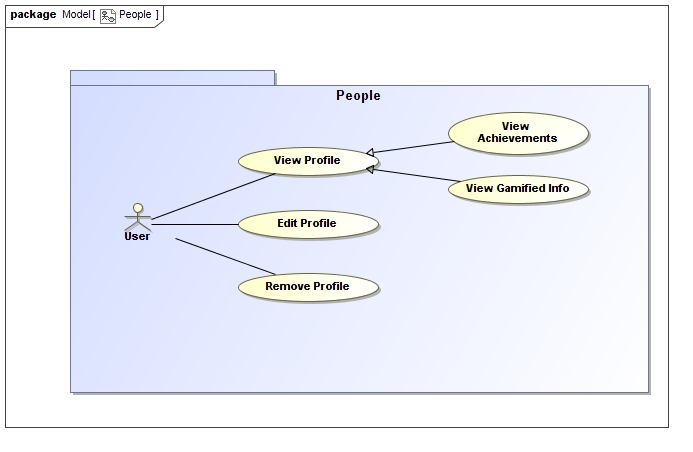
\includegraphics[width=\textwidth]{../software-architecture-specification/People.jpg}
			\caption{The scope of functionality required from the \emph{People} module}
		\end{figure}
		
		The scope of the \emph{People} module includes:
		
		\begin{itemize}
			\item Letting a user view their profile, on which will be achievements and gamified information (like badges and progress).
			\item Allowing a user to edit their profile information.
			\item Deleting of profiles.
		\end{itemize}
		
	\pagebreak
	\subsection{Analytics}
		The scope of the \emph{Analytics} module is shown below in Figure 3.
		
		\begin{figure}[H]
			\centering
			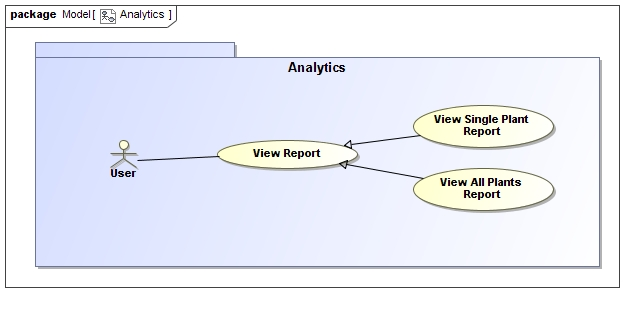
\includegraphics[width=\textwidth]{../software-architecture-specification/Analytics.jpg}
			\caption{The scope of functionality required from the \emph{Analytics} module}
		\end{figure}
		
		The scope of the \emph{} module includes:
		
		\begin{itemize}
			\item Viewing reports of either a single plant or a summary of all plant details.
		\end{itemize}
		
	\pagebreak
	\subsection{Notifications}
		The scope of the \emph{Notifications} module is shown below in Figure 4.
		
		\begin{figure}[H]
			\centering
			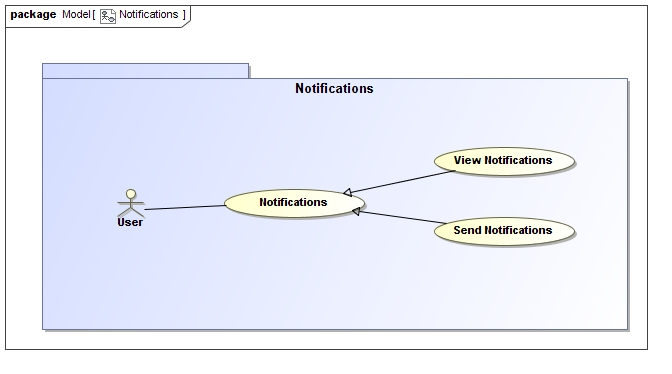
\includegraphics[width=\textwidth]{../software-architecture-specification/Notifications.jpg}
			\caption{The scope of functionality required from the \emph{Notifications} module}
		\end{figure}
		
		The scope of the \emph{} module includes:
		
		\begin{itemize}
			\item Viewing received notifications.
			\item Sending notifications to other users.
		\end{itemize}

\section{Functional Requirements and Application Design}
	\subsection{Use Case Prioritization}
		\subsubsection{Critical}
			\begin{itemize}
				\item User Management Subsystem:
				\begin{itemize}
					\item Register Account
					\item Login
				\end{itemize}
				
				\item Plant/Device Management Subsystem:
				\begin{itemize}
					\item Create Plant
					\item View Plant Status
				\end{itemize}
				
				\item Device Communications Subsystem
				\begin{itemize}
					\item Send Updated Settings/Configuration to Device
					\item Send Readings Summary to Lambda
				\end{itemize}
			\end{itemize}
			
		\subsubsection{Important}
		\begin{itemize}
			\item User Management Subsystem:
			\begin{itemize}
				\item Edit Details
				\item View Gamification Info
			\end{itemize}
			
			\item Plant/Device Management Subsystem:
			\begin{itemize}
				\item Edit Plant Details
				\item Add Sensor to Device
				\item Remove Sensor from Device
				\item Edit Plant Configuration/Settings
				\item Remove Plant
			\end{itemize}
		\end{itemize}
	
\cleardoublepage

	\subsection{Use Case/Services Contracts}
		\subsubsection{User Management Subsystem}
			\begin{figure}[H]
				\centering
				\includegraphics[width=\textwidth]{../images/user-management-subsystem.png}
				\caption{The \emph{User Management} subsystem}
			\end{figure}
		\paragraph{Register Account}
			A user should be able to register an account using the \emph{Register Account} page. The user should not be able to log in before they have registered. Once the user has registered an account, they should be able to \emph{Log In (1.2)}.
			\begin{figure}[H]
				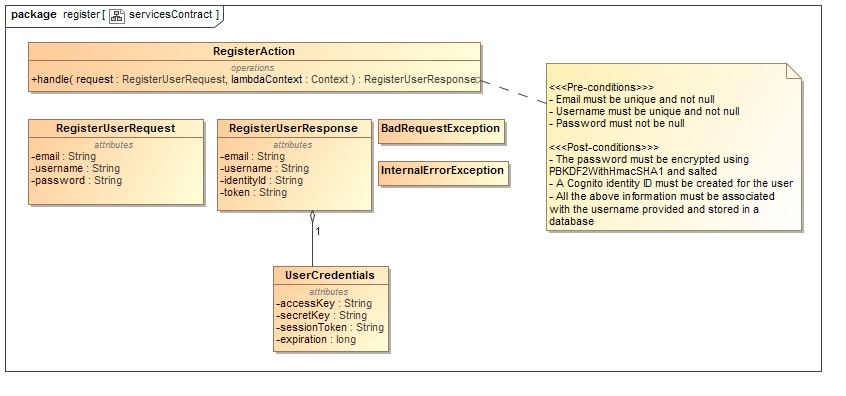
\includegraphics[width=\linewidth]{../images/ServicesContracts/register.jpg}
				\caption{Services Contract - Register User}
			\end{figure}
			
\cleardoublepage
		\paragraph{Log In}
			Once a user has been registered, the user should be able to log into their account. They cannot log in before registering. They have to provide the correct username and password in order to log in. Once the correct credentials have been given, they are taken to the \emph{Home Page} where they can \emph{Edit Details (1.3)}, \emph{View Gamification Information (1.4)} and access the \emph{Plant/Device Management Subsystem (2)}.
			\begin{figure}[H]
				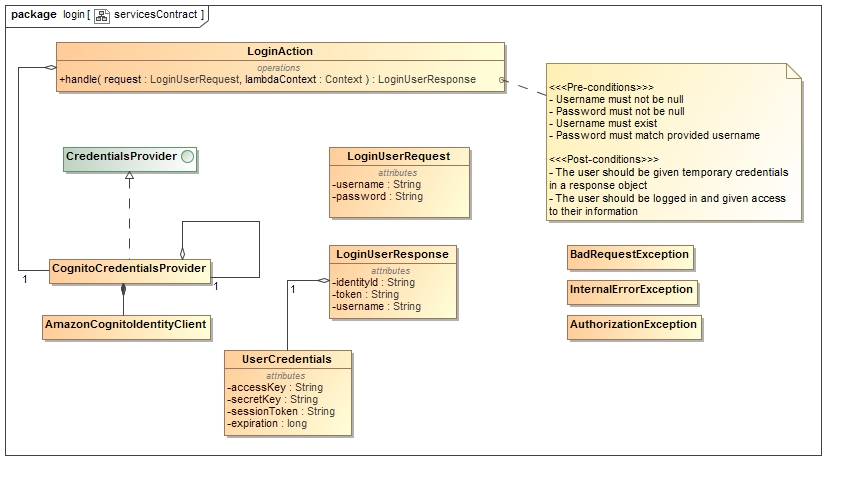
\includegraphics[width=\linewidth]{../images/ServicesContracts/login.jpg}
				\caption{Services Contract - Login User}
			\end{figure}
		\paragraph{Edit Details}
			Once a user has logged in, they can edit their details from the \emph{Edit Details} page. They can change their email, password and other personal details, but cannot change their username. They can then save the changes and they will take effect immediately.
		\paragraph{View Gamifaction Information}
			Once a user has logged in, they can view their current gamification information. This will show them their standings in the leaderboards, the awards and badges they have achieved and progress to following markers.			
	
\cleardoublepage
		\subsubsection{Plant/Device Management Subsystem}
			\begin{figure}[H]
				\centering
				\includegraphics[width=\textwidth]{../images/plant-management-subsystem.png}
				\caption{The \emph{Plant Management} subsystem}
			\end{figure}
			\paragraph{Create Plant}
			The user should be able to create a plant on their account. Through this, they can add the device the plant is connected to, add the type of plant, select which sensors are connected to the plant etc.
			\begin{figure}[H]
				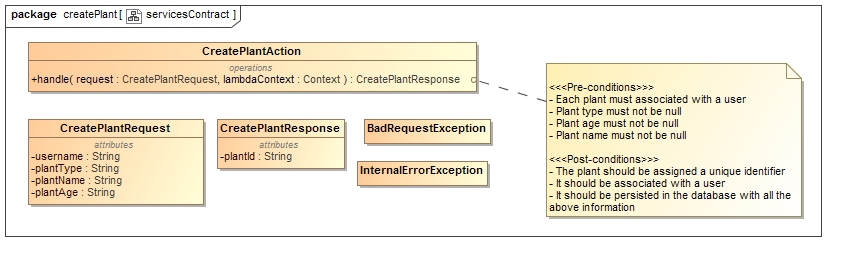
\includegraphics[width=\linewidth]{../images/ServicesContracts/createPlant.jpg}
				\caption{Services Contract - Create Plant}
			\end{figure}
			
\cleardoublepage
			\paragraph{View Plant Status}
			The user should be able to view the status of their existing plants. This page will show the most recent data collected by the device as well as historical data for a specific plant. The date of the data is dislpayed and the user has the option of requesting a forced update from the device.
			\paragraph{Update Plant Details}
			The user should be able to edit the details of an existing plant. They can change the basic information (type of plant etc) as well as \emph{Add Sensor to Device (2.4)}, \emph{Remove Sensor from Device (2.5)} and \emph{Edit Plant Configuration/Settings (2.6)}.
			\begin{figure}[H]
				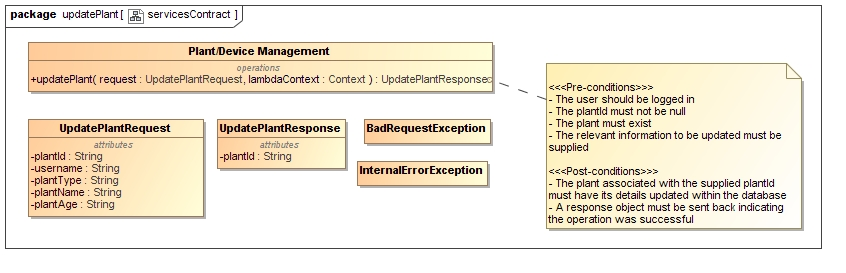
\includegraphics[width=\linewidth]{../images/ServicesContracts/updatePlant.jpg}
				\caption{Services Contract - Update Plant}
			\end{figure}
			\paragraph{List User Plants}
			The user should be able to request a list of the plants associated with their account.
			\begin{figure}[H]
				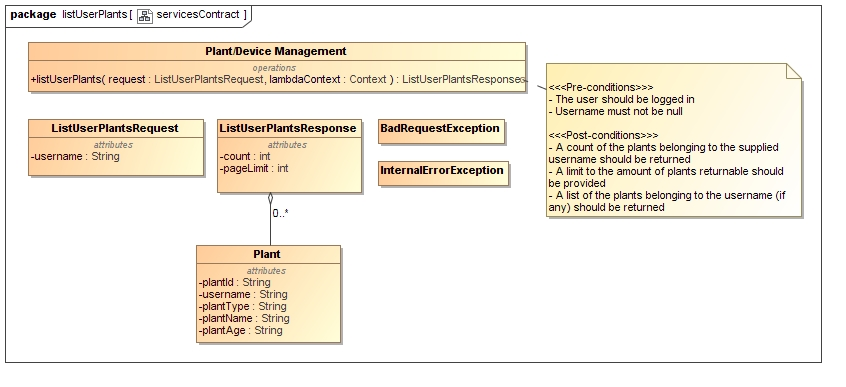
\includegraphics[width=\linewidth]{../images/ServicesContracts/listUserPlants.jpg}
				\caption{Services Contract - List User Plants}
			\end{figure}
			
\cleardoublepage
			\paragraph{Add Sensor to Device}
			The user should be able to select a device and add a sensor to the device.
			\paragraph{Remove Sensor from Device}
			The user should be able to select a device and remove a sensor from the device. The removed sensor should not be removed from the historical view, but will not be shown on the \emph{View Plant Status (2.2)} and the \emph{Edit Plant Configuration/Settings (2.6)} pages.
			\paragraph{Edit Plant Configuration/Settings}
			The user should be able to select a plant and edit the current configuration for the configurable settings on the device. This includes water cycles, light settings, air flow etc.
			\paragraph{Remove Plant}
			The user should be able to remove a plant. This will disable the connected device and disable the \emph{View Plant Status (2.2)} and the \emph{Edit Plant Configuration/Settings (2.6)} pages for that plant, but the plant should still be in the historical view.
			\begin{figure}[H]
				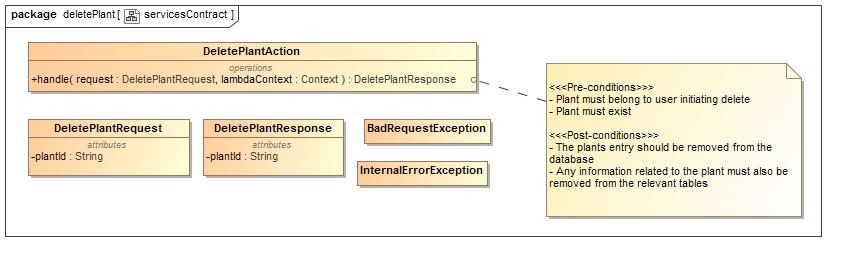
\includegraphics[width=\linewidth]{../images/ServicesContracts/deletePlant.jpg}
				\caption{Services Contract - Delete Plant}
			\end{figure}
		
\cleardoublepage
		\subsubsection{Device Communications Subsystem}
		\begin{figure}[H]
			\centering
			\includegraphics[width=\textwidth]{../images/device-communications-subsystem.png}
			\caption{The \emph{Device Communications Subsystem} subsystem}
		\end{figure}
		\paragraph{Send Updated Settings/Configuration to Device}
			The Lambda server should be able to send settings set in the \emph{Edit Plant Configuration/Settings (2.6)} page and send them to the device. This is done by updating the device shadow and synchronising the device with its shadow.
		\paragraph{Send Readings Summary to Lambda}
			On a regular schedule, the device should send its summary of readings from the sensors to the Lambda server. The subscribed users can then view the summary in the \emph{View Plant Status (2.2)} page and historical summary.

\cleardoublepage		
	
	\subsection{Process Specifications}
		\subsubsection{Create Plant Use Case}
			\begin{figure}[H]
				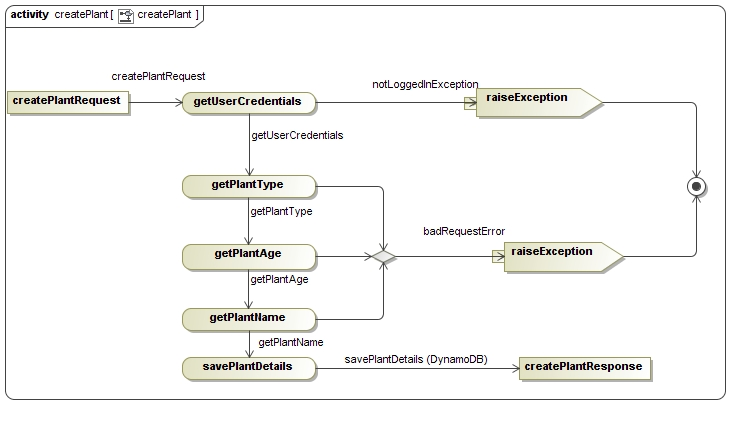
\includegraphics[width=\linewidth]{createPlant.jpg}
				\caption{Activity Diagram for the Create Plant use case}
			\end{figure}
	\newpage
		\subsubsection{Update Plant Use Case}
			\begin{figure}[H]
				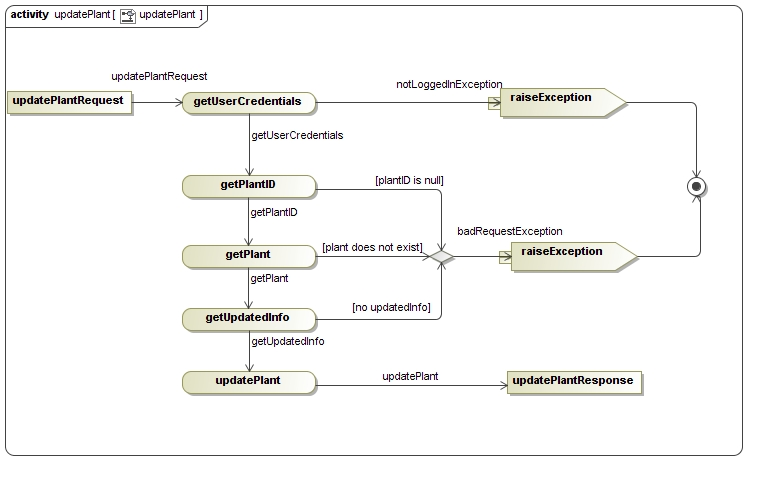
\includegraphics[width=\linewidth]{updatePlant.jpg}
				\caption{Activity Diagram for the Update Plant use case}
			\end{figure}
	\newpage
		\subsubsection{Delete Plant Use Case}
			\begin{figure}[H]
				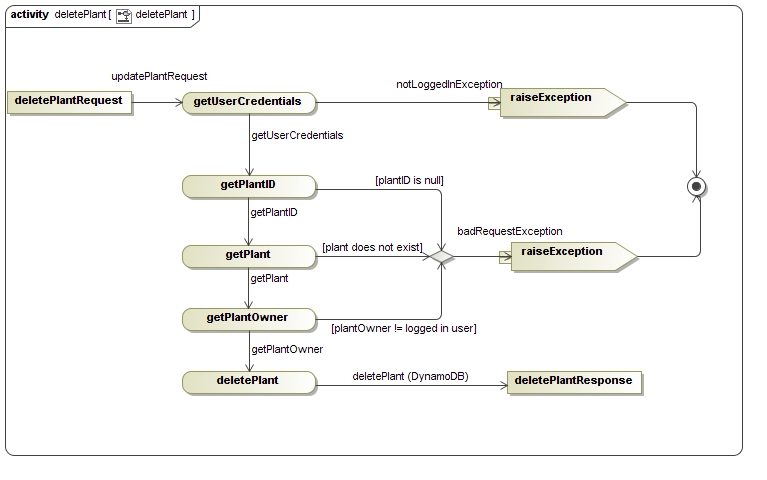
\includegraphics[width=\linewidth]{deletePlant.jpg}
				\caption{Activity Diagram for the Delete Plant use case}
			\end{figure}
	\newpage
		\subsubsection{Device Update Status Use Case}
			\begin{figure}[H]
				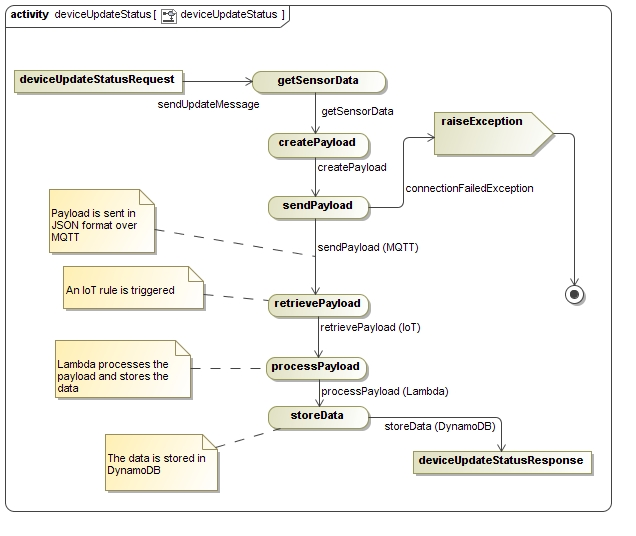
\includegraphics[width=\linewidth]{deviceUpdateStatus.jpg}
				\caption{Activity Diagram for the Device Update Status use case}
			\end{figure}
	\newpage
	
	\begin{landscape}
		\subsection{Domain Model}
		\begin{figure}[H]
			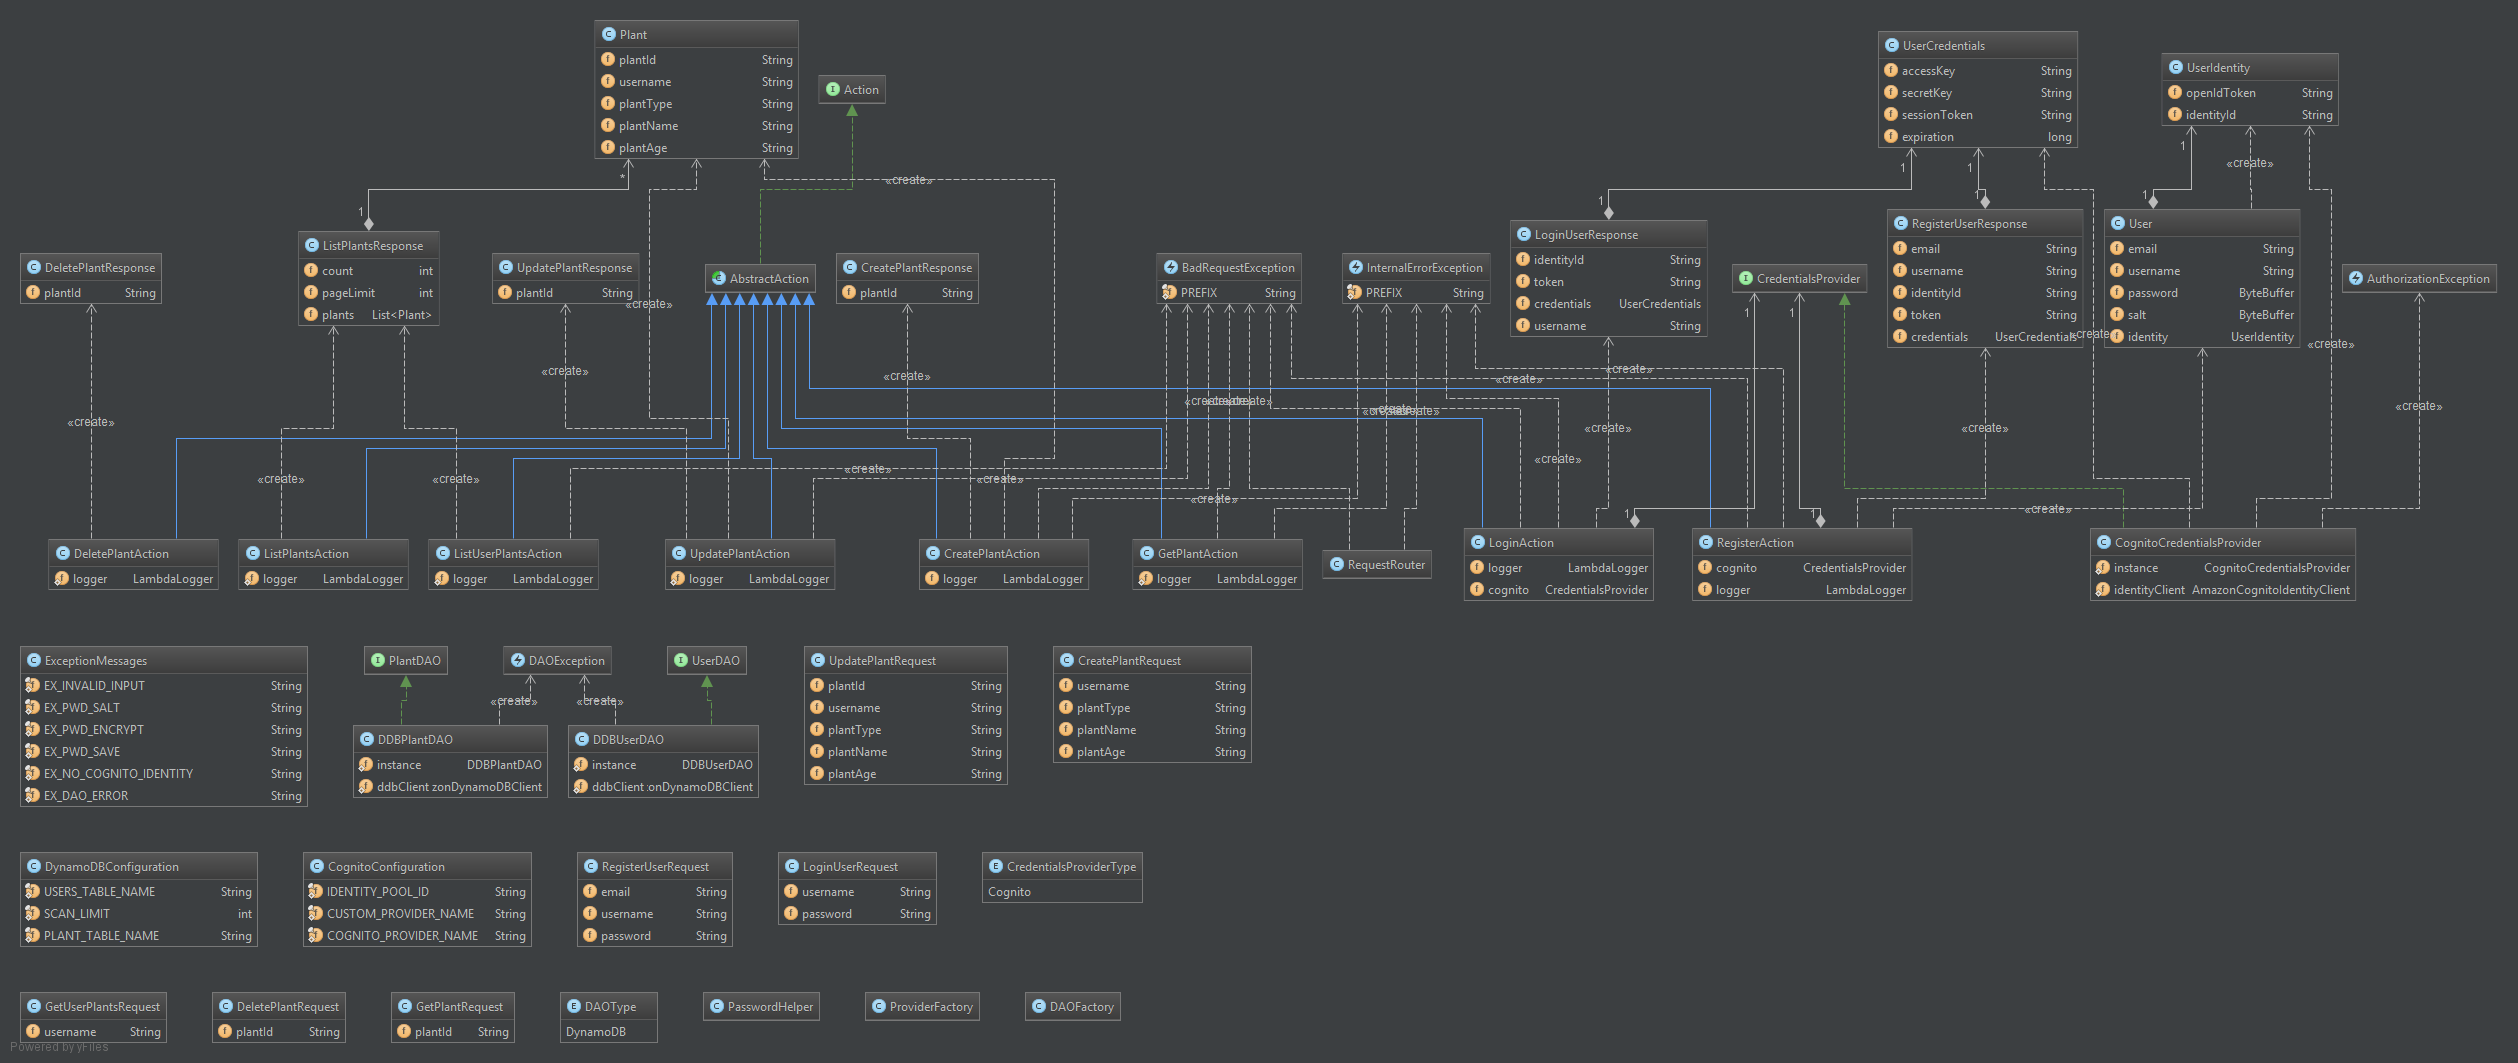
\includegraphics[width=\linewidth]{../images/aworldofplants_domain.png}
			\caption{Domain model}
		\end{figure}
	\end{landscape}

\newpage
\section{Open Issues}
	\begin{itemize}
		\item What is the process to be followed when adding a new device?
		\begin{itemize}
			\item The device needs the code and certificates uploaded to it
			\item As much as possible needs to be automated for the user. Detailed steps should be given
		\end{itemize}

		\item How do you rate the conditions of the plants?
		Ideas:
		\begin{itemize}
			\item Using a colour palette to measure the leaf colour
			\item Getting the user to enter his analysis of the state of the plant
		\end{itemize}

		\item What type of gamification elements are going to be present?

	\end{itemize}
\end{document}